\subsection{Conditioning input data}
\label{sec:conditioningExperiments}

\subsubsection{Frequency Analysis}
	We use \verb!MATLAB!\textsuperscript{\textregistered}'s function \verb|spectrogram|, which takes the following parameters
	\begin{itemize}
		\item \verb!X! -- our signal $\vec x = \{x_1, x_2, \dotsc, x_N\}$.
		\item \verb!WINDOW! -- length (in number of samples) of the window $T_\text{window}$. The windows are automatically filtered using a Hamming window. We arbitrarily choose the window to be the number of signal samples corresponding to one annotation (6000 in our case).
		\item \verb!NOVERLAP! -- number of overlapping samples between two consecutive windows. Effectively $T_\text{window} - T_\text{offset}$. We arbitrarily choose the offset to be 1000 such that we have six bins of PSD's for each annotation.
		\item \verb!NFFT! -- number of frequency points used to calculate the discrete Fourier transforms. We use default.
		\item \verb!Fs! -- sampling frequency in Hz. In our case 100 Hz.
	\end{itemize}

	A spectrogram for one record can be seen in Figure \ref{fig:visualiseSpectrogram}. Just by looking at the spectrogram, we can spot different regimes of the time series (most clearly seen at $0.5 \times 10^4$, $1 \times 10^4$, $2 \times 10^4$, and $2.7 \times 10^4$ seconds). Comparing this to the apnoea annotations in Figure \ref{fig:visualiseData}, these regimes are actually the non-apnoeatic regimes. Also, we can see that most of the ``action'' is happening below 20 Hz. For this reason, we cut off the frequencies above 25 Hz for subsequent analysis. We combine the corresponding six bins of PSD's per annotation in to a large feature vector corresponding to that annotation. Next, we will reduce the dimensionality of these feature vectors using PCA.
	\begin{figure}[ht!]
		\centering
			\includegraphics[width=.5\textwidth]{drawings/visualiseSpectrogram.eps}
		\caption{Spectrogram of one record}
		\label{fig:visualiseSpectrogram}
	\end{figure}

\subsubsection{PCA}
	For this, we use the function \verb!pca! from the package \verb!pmtk3!. Once we get the principal components (orthogonal bases) and their corresponding principal coefficients (variances of the data, projected onto that base, correct to a constant factor) $\{\lambda_1, \lambda_2, \dotsc, \lambda_D\}$, we will plot the graph of their cumulative sum over their total sum $\frac{\sum_{i = 1}^n \lambda_i}{\sum_{j = 1}^N \lambda_j}$ in order to decide on the number of principal components needed. The plot is in the Figure \ref{fig:visualisePca}. Performed on the first 10 records, we can see that we will need to include at least 100 to capture half of the variance but at least 3000 components to capture the whole variance.
	\begin{figure}[ht!]
		\centering
			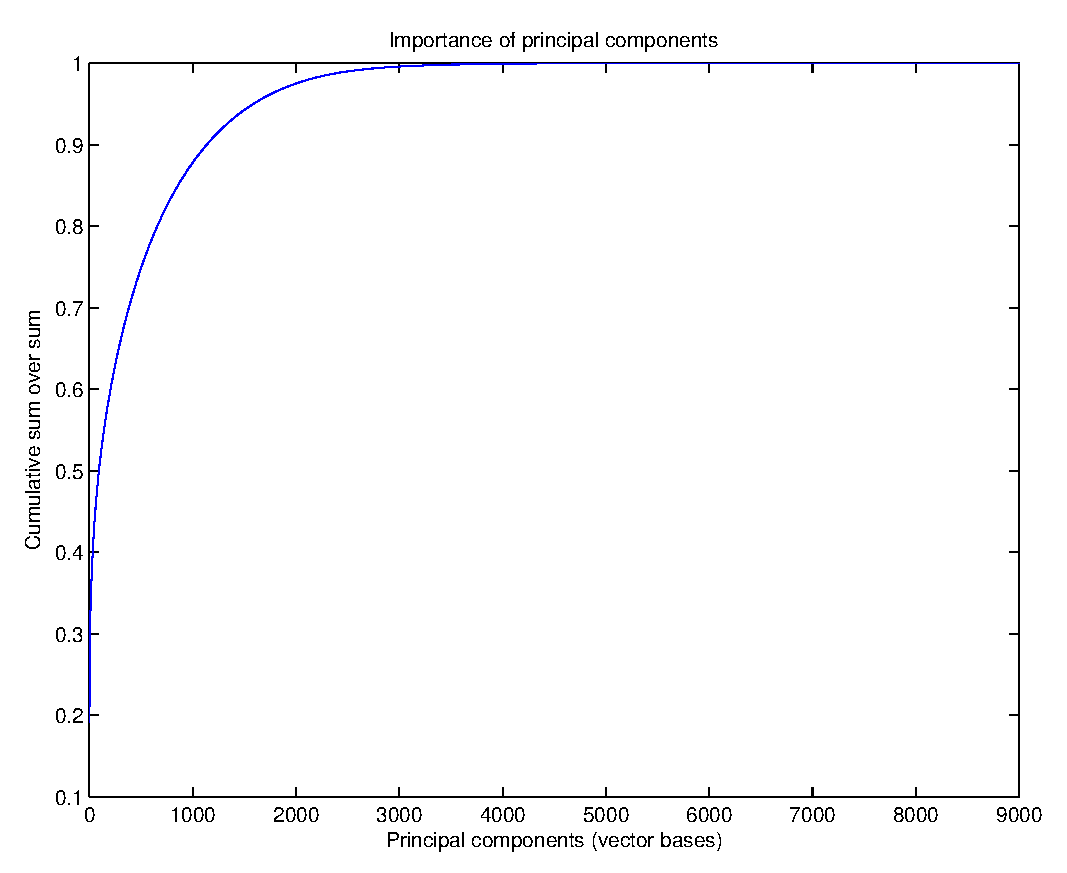
\includegraphics[width=.5\textwidth]{drawings/visualisePca.eps}
		\caption{PCA of the first 10 records}
		\label{fig:visualisePca}
	\end{figure}